\documentclass[14pt,letterpaper]{article}
\usepackage[utf8]{inputenc}
\title{EV 1.6 EXPLICAR LA OPERACION DE LOS CIRCUITOS DE ACTIVACION CON TIRISTORESEN CONVERTIDORES CA-CD, CA-CA}
\author{Ascencio De Leon Agustin}
\usepackage[spanish]{babel}
\usepackage{graphicx}
\graphicspath{{imagenes2/}}
\usepackage[left=2.5cm,top=2.5cm,bottom=3cm,right=2.5cm]{geometry}


\begin{document}
\maketitle
\begin{figure}[h!]
\centering
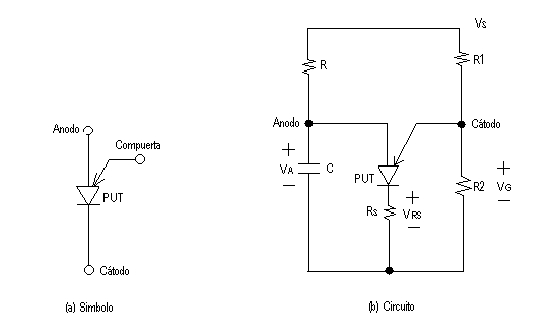
\includegraphics[scale=.9]{inicio}
\end{figure}
\newpage
\section{¿que es un tiristor?}
El tiristor es un semiconductor de potencia que se utiliza como interruptor, ya sea para conducir o interrumpir la corriente eléctrica, a este componente se le conoce como de potencia por que se utilizan para manejar grandes cantidades de corriente y voltaje, a comparación de los otros semiconductores que manejan cantidades relativamente bajas.
Cuando se habla de tiristores comúnmente se cataloga al tiristor como un SRC (silicon controlled rectifier), pero esto no es del todo correcto ya que este tipo es el más popular y conocido pero no es el único que existe.



\section{¿como funciona un tiristor?}
Los tiristores están conformados por 3 terminales un ánodo, un cátodo y una compuerta o mejor conocida “gate”, su funcionamiento se asemeja al de un relevador o un interruptor mecánico, Ya que cuando aplicas una corriente a la terminal gate este se activa y obtiene la característica de dejar pasar a la electricidad.

\section{tipos de tiristor}
De control de fase o comunicación rápida (SCR)
Este tipo es el más común y más utilizado, debido a que son capaces de conmutar rápidamente. Una de las características principales de este tiristor es que solo es capaz de conducir electricidad hacia una sola dirección (como un diodo cuando se polariza directamente), una vez activado este componente no importa si quitas la corriente de la puerta ya que este seguirá activo hasta que se cumpla una de dos condiciones posibles. Para desactivarlo tenemos que cortar el suministro de corriente o llevarla hasta un punto muy bajo que el tiristor sea incapaz de seguir conduciendo.
\linebreak 
\linebreak
Bidireccionales controlados por face (BCT):
Este tipo corresponde a dos tiristores en un mismo encapsulado, aun que están juntos no interfieren entre si cada uno tiene sus terminales puerta para ser activados.
\linebreak
\linebreak
Fototiristor (LASCR):
Este como su nombre lo indica es un tiristor el cual se activa mediante la luz.
\linebreak
\linebreak
Triodo bidireccional (TRIAC):
Se usa para la corriente alterna ya que contiene dos tiristores juntos  en un mismo encapsulados, en este ocasión solo cuentan con una terminal puerta y esta es capaz de activar a los dos componentes al mismo tiempo. 
\linebreak
\linebreak
De conducción inversa (RCT)
Se podría decir que es un SCR con la integración de un diodo colocado en paralelo pero inversamente, esto se utiliza para evitar que corrientes parásitas generadas debido a inducciones circulen en contra flujo de la corriente.
\linebreak
\linebreak
De desactivación por compuerta (GTO)
Este tipo es una mejora del tiristor SCR ya que puede desactivarse travez de su puerta con la única condición de aplicar voltaje negativo.

etc.etc.etc...
\newpage
\section{¿que es un circuito de potencia?}
El circuito de disparo o excitación de compuerta de los tiristores, es una parte integral
del convertidor de potencia. La salida de un convertidor, que depende de la forma en
que el circuito de disparo excita a los dispositivos de conmutación (tiristores), es una
función directa del proceso de cómo se desarrolla la conmutación. Podemos decir
entonces que los circuitos de disparo, son elementos claves para obtener la salida
deseada y cumplir con los objetivos del “sistema de control”, de cualquier convertidor
de energía eléctrica.
\linebreak
\linebreak
\linebreak
\section{partes componentes de un circuito de disparo para tiristores}
Las partes componentes de un circuito de disparo para tiristores usados en los
rectificadores controlados por fase, a frecuencia industrial, son los siguientes: El
circuito sincronizador, el circuito base de tiempo para retrasar el disparo, el circuito
conformador del pulso, el circuito amplificador del pulso (opcional), el circuito aislador
y finalmente el circuito de protección de la compuerta del tiristor.
\newpage
\section{como funcina un circuito de activacion(de disparo)}
acelera la conmutación al corte de transistores con puerta tipo Bipolar ó
MOS puede aplicarse una tensión negativa en la puerta, así:
3/4 En los BJT, aparece una corriente de base negativa que disminuye
drásticamente el tiempo de almacenamiento.
3/4 En los MOS e IGBT se acelera la descarga de la capacidad de puerta como se
observa en la siguiente figura:
\begin{figure}[h!]
\centering
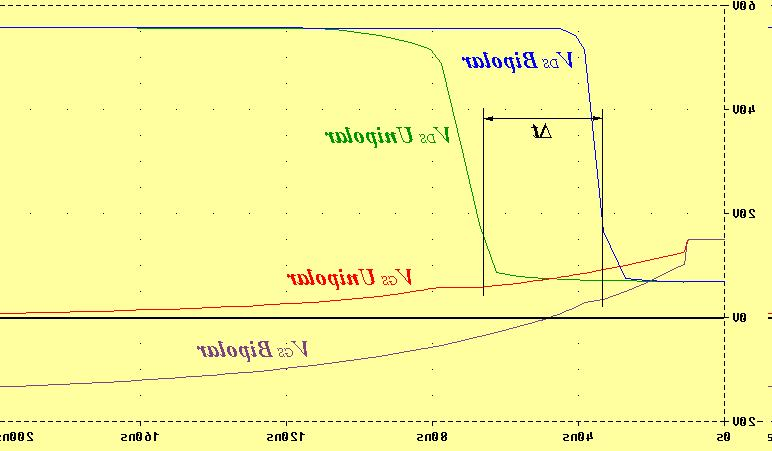
\includegraphics[scale=.4]{f}

\end{figure}
La tensión Vcc vale 55Volt., la resistencia de puerta es de 50 Ohmios y la
tensión VGS vale inicialmente +20Volt. cambiando a 0Volt. en el caso
Unipolar y a –20Volt. en el caso Bipolar. El retraso que se observa entre
ambos casos es de unos 35nS.
\linebreak
\linebreak
\linebreak
\linebreak
\section{¿cual es su funcion?}
la funcion de un circuito de activacion es mandar una carga de voltaje controlada a un controlador, dando como resultado un "disparo". el cual ejecuta una accion.
\newpage
\section{bibliografias}
$
https://www.academia.edu/7728470/CIRCUITOS_DE_DISPARO_DE_TIRISTORES_PARA_RECTIFICADORES_CONTROLADOS
\linebreak
https://ingenieriaelectronica.org/circuitos-de-activacion-para-diodos-laser/
\linebreak
https://www.ingmecafenix.com/electronica/que-es-un-tiristor-y-como-funciona/
\linebreak
http://www.gte.us.es/~leopoldo/Store/tsp_9.pdf
$




\end{document}